\documentclass{mem}
\usepackage{natbib}\usepackage{txfonts}\usepackage{balance}
\usepackage{graphicx}
\usepackage[a4paper,breaklinks,dvipdfm]{hyperref}
\idline{75}{282}
\begin{document}
\def\teff{$T\rm_{eff }$}
\def\kms{$\mathrm {km s}^{-1}$}

\title
{Mapping young stellar populations towards Orion with \textit{Gaia} DR1}

   \subtitle{}

\author{
E. \,Zari\inst{1} 
\and A.G.A. \, Brown\inst{1}
          }

 

\institute{
Leiden Observatory, Niels Bohrweg 2, 2333 CA Leiden, the Netherlands \\ email: {\tt zariem@strw.leidenuniv.nl}}

\authorrunning{Zari et al.}


\titlerunning{Mapping young stellar populations towards Orion with \textit{Gaia} DR1}


\abstract{
OB associations are prime sites for the study of star formation
processes and of the interaction between young massive stars with
the interstellar medium. Furthermore, the kinematics and structure of
the nearest OB associations provide detailed insight into the properties
and origin of the Gould Belt.
In this context, the Orion complex has been extensively studied.
However, the spatial distribution of the stellar population is still
uncertain: in particular, the distances and ages of the various
sub-groups composing the Orion OB association, and their connection to
the surrounding interstellar medium, are not well determined.
We used the first \textit{Gaia} data release to characterize the stellar
population in Orion, with the goal to obtain new distance and age
estimates of the numerous stellar groups composing the Orion OB
association. We found evidence of the existence of a young and rich
population spread over the entire region, loosely clustered around some
known groups. This newly discovered population of young stars provides a
fresh view of the star formation history of the Orion region.
\keywords{Stars: distances - stars: formation - stars: pre-main sequence - stars: early-type}
}
\maketitle{}

\section{Introduction}
OB stars are not distributed randomly in the sky, but cluster in loose, unbound groups, which are usually referred to as OB associations \citep[]{Blaauw1964}.
In the solar vicinity, OB associations are located near star-forming regions \citep[]{Bally2008}, hence they are prime sites for large scale studies of star formation processes and of the effects of early-type stars on the interstellar medium. 
The Orion star forming region is the nearest ($d \sim 400 \, \mathrm{pc}$) giant molecular cloud complex. All stages of star formation can be found here, from protoclusters, to OB associations \cite[]{Brown1994, Bally2008, Briceno2008, Muench2008, DaRio2014}. The different modes of star formation occurring here (isolated, distributed, and clustered) allow us to study  the effect of the environment on star formation processes in great detail. Moreover, the Orion region is an excellent nearby example of the effects that young, massive stars have on the surrounding interstellar medium \citep[]{Ochsendorf2015, Schlafly2015}. 
The Orion OB association (Ori OB1) consists of several groups, with different ages, partially superimposed along our line of sight \citep[]{Bally2008} and extending over an area of $\sim 30^{\circ} \times 25^{\circ}$.
We use the first \textit{Gaia} data release \citep[]{Brown2016, Prusti2016}, hereafter \textit{Gaia} DR1, to explore the three dimensional arrangement and the age ordering of the many stellar groups towards Orion, with the overall goal to construct a new classification and characterization of the stellar population in the region.  
Our approach is based on the parallaxes provided in the \textit{Tycho-Gaia Astrometric Solution} \citep[TGAS]{Michalik2015, Lindegren2016}, a sub-set of the \textit{Gaia} DR1 catalogue, and on the combination of \textit{Gaia} DR1 and 2MASS photometry.  
\begin{figure}
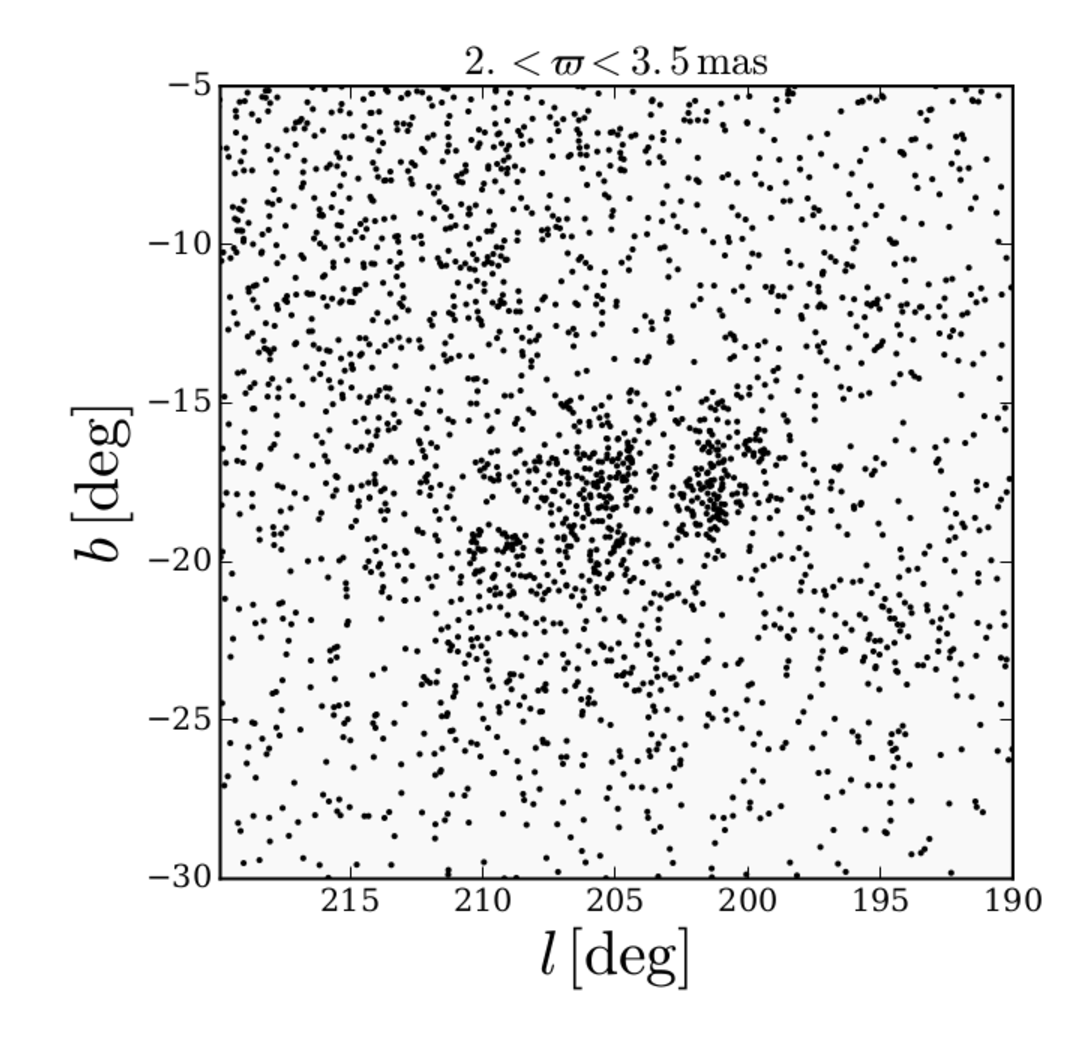
\includegraphics[width = \hsize]{fig5a_cut.eps}
\caption{Positions in the sky of the TGAS sources selected with Eq. (1), and with parallax $ 2 < \varpi <3.5 \, \mathrm{mas}$. }
\label{fig1}
\end{figure}


\section{Orion in \textit{Gaia} DR1}
We first consider all the TGAS sources in the field.
Since the  motion of Orion OB1 is mostly directed radially away from the Sun, the observed proper motions are small. For this reason, a rough selection of the TGAS sources can be made requiring:
\begin{equation}\label{eq3}
(\mu_{\alpha*} - 0.5)^2 + (\mu_{\delta}+1)^2 < 25  \,\mathrm{mas^2 \, yr^{-2}},
\end{equation}
where $\mu_{\alpha*}$ and $\mu_{\delta}$ are the proper motions in right ascension and declination. 
Fig. \ref{fig1} shows the distribution  in the sky of the sources  with parallax $2 < \varpi < 3.5 \, \mathrm{mas}$, which corresponds to a distance $285 < d < 500 \, \mathrm{pc}$. 
Some source over-densities towards the center of the field, $(l, b) \sim (205^{\circ}, -18^{\circ})$, are clearly visible, and they are not due to projection effects but are indicative of real clustering in three dimensional space. 
%The stars within the density enhancements of Fig. 1 also show a small gradient in the parallax - galactic longitude plane. In particular, the stars associated with 25 Ori have slightly larger parallaxes than those in the direction towards the ONC.

We combine \textit{Gaia} and 2MASS photometry to construct color-magnitude diagrams (CMD) of the sources within the density enhancements. Fig. 2 shows the $G$ vs. $G-J$ CMD of the field. The big black points represent the TGAS sources within the density enhancements of Fig. 1, while the small black dots are the \textit{Gaia} DR1 sources. The TGAS sources define a sequence at the bright end of the CMD, whose faint counterpart is visible between $G = 14 \, \mathrm{mag}$ and $G = 18 \, \mathrm{mag}$. The latter might indicate the presence of a population of young stars, since it is situated above the main sequence at the distance of Orion. To clean our sample, we first
excluded the bulk of the field stars by requiring (orange line in Fig. 2):
$G < 2.5(G-J)$ + 10.5 for  $G > 15$ mag,
$G < 2.9\,(G-J)$ + 9.9 for $G < 15$ mag.
\noindent
\begin{figure}
\includegraphics[width = \hsize]{fig62.eps} \\
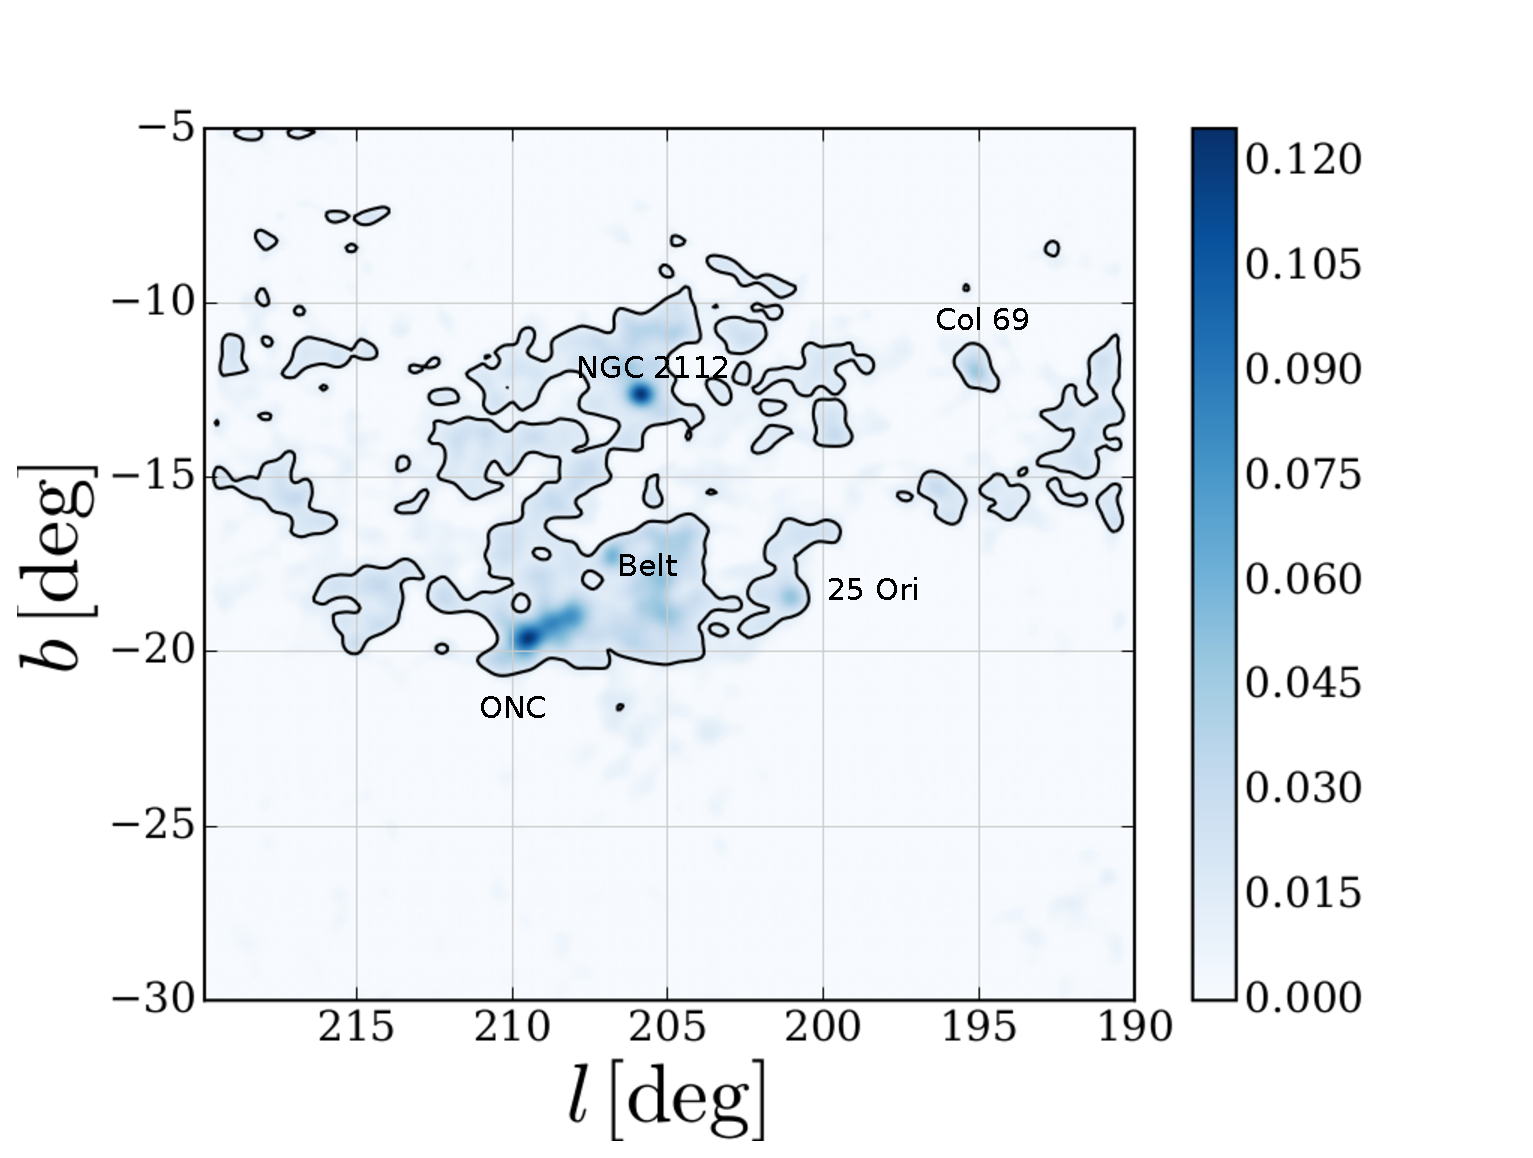
\includegraphics[width = \hsize]{fig4.eps}
\caption{Top: Colour magnitude diagram of the \textit{Gaia} DR1 sources cross-matched with 2MASS.  Bottom: Background subtracted normalized probability density function of the stars selected with with Eq. 2.}
\label{fig3}
\end{figure}
Then we analyse the distribution in the sky of the remaining sources using  a multivariate normal kernel, with isotropic  bandwidth = $0.3^{\circ}$.
Fig. 2 (bottom) shows the background subtracted normalized density function of the source distribution. The groups clearly separate from the field stars. We further select all the sources within the contour levels shown in Fig. 2, and we determine their ages with a Bayesian isochrone fitting procedure  \citep[]{JL05} and  \citep[]{Valls-Gabaud2014}, fixing the parallax to $\varpi = 2.65 \, \mathrm{mas}$. This value corresponds to the mean parallax for the TGAS sources within the density enhancements shown in Fig. 1.
%We compare the observed $G$ magnitude and $G-J$ color to those predicted by the PARSEC  (PAdova and TRieste Stellar Evolution Code, \cite[Bressan et al. 2012]{Bressan2012}, \cite[Chen et al. 2014]{Chen2014}, \cite[Tang et al. 2014]{Tang2014}) library of stellar evolutionary tracks.
%We applied an extinction correction of $A_V = 0.25 \,  \mathrm{mag}$ and we fixed the metallicity to $Z = 0.02$, following \cite{Brown1994}.
%We fixed the parallax to $\varpi = 2.65 \, \mathrm{mas}$, which correspond to the mean parallax for the TGAS sources within the density enhancements.
Fig. 2 (bottom) shows the density (Gaussian kernel, with bandwidth = $0.5^{\circ}$) of the source sky distribution as a function of their age, $t$.  
The coordinates of the density enhancements change with time. This means that the groups we identified have different relative ages.
The last panel shows the stars with estimated ages $> 20$ Myr. These are field stars: their distribution is almost uniform, and their density increases towards the Galactic plane. 
\begin{figure}
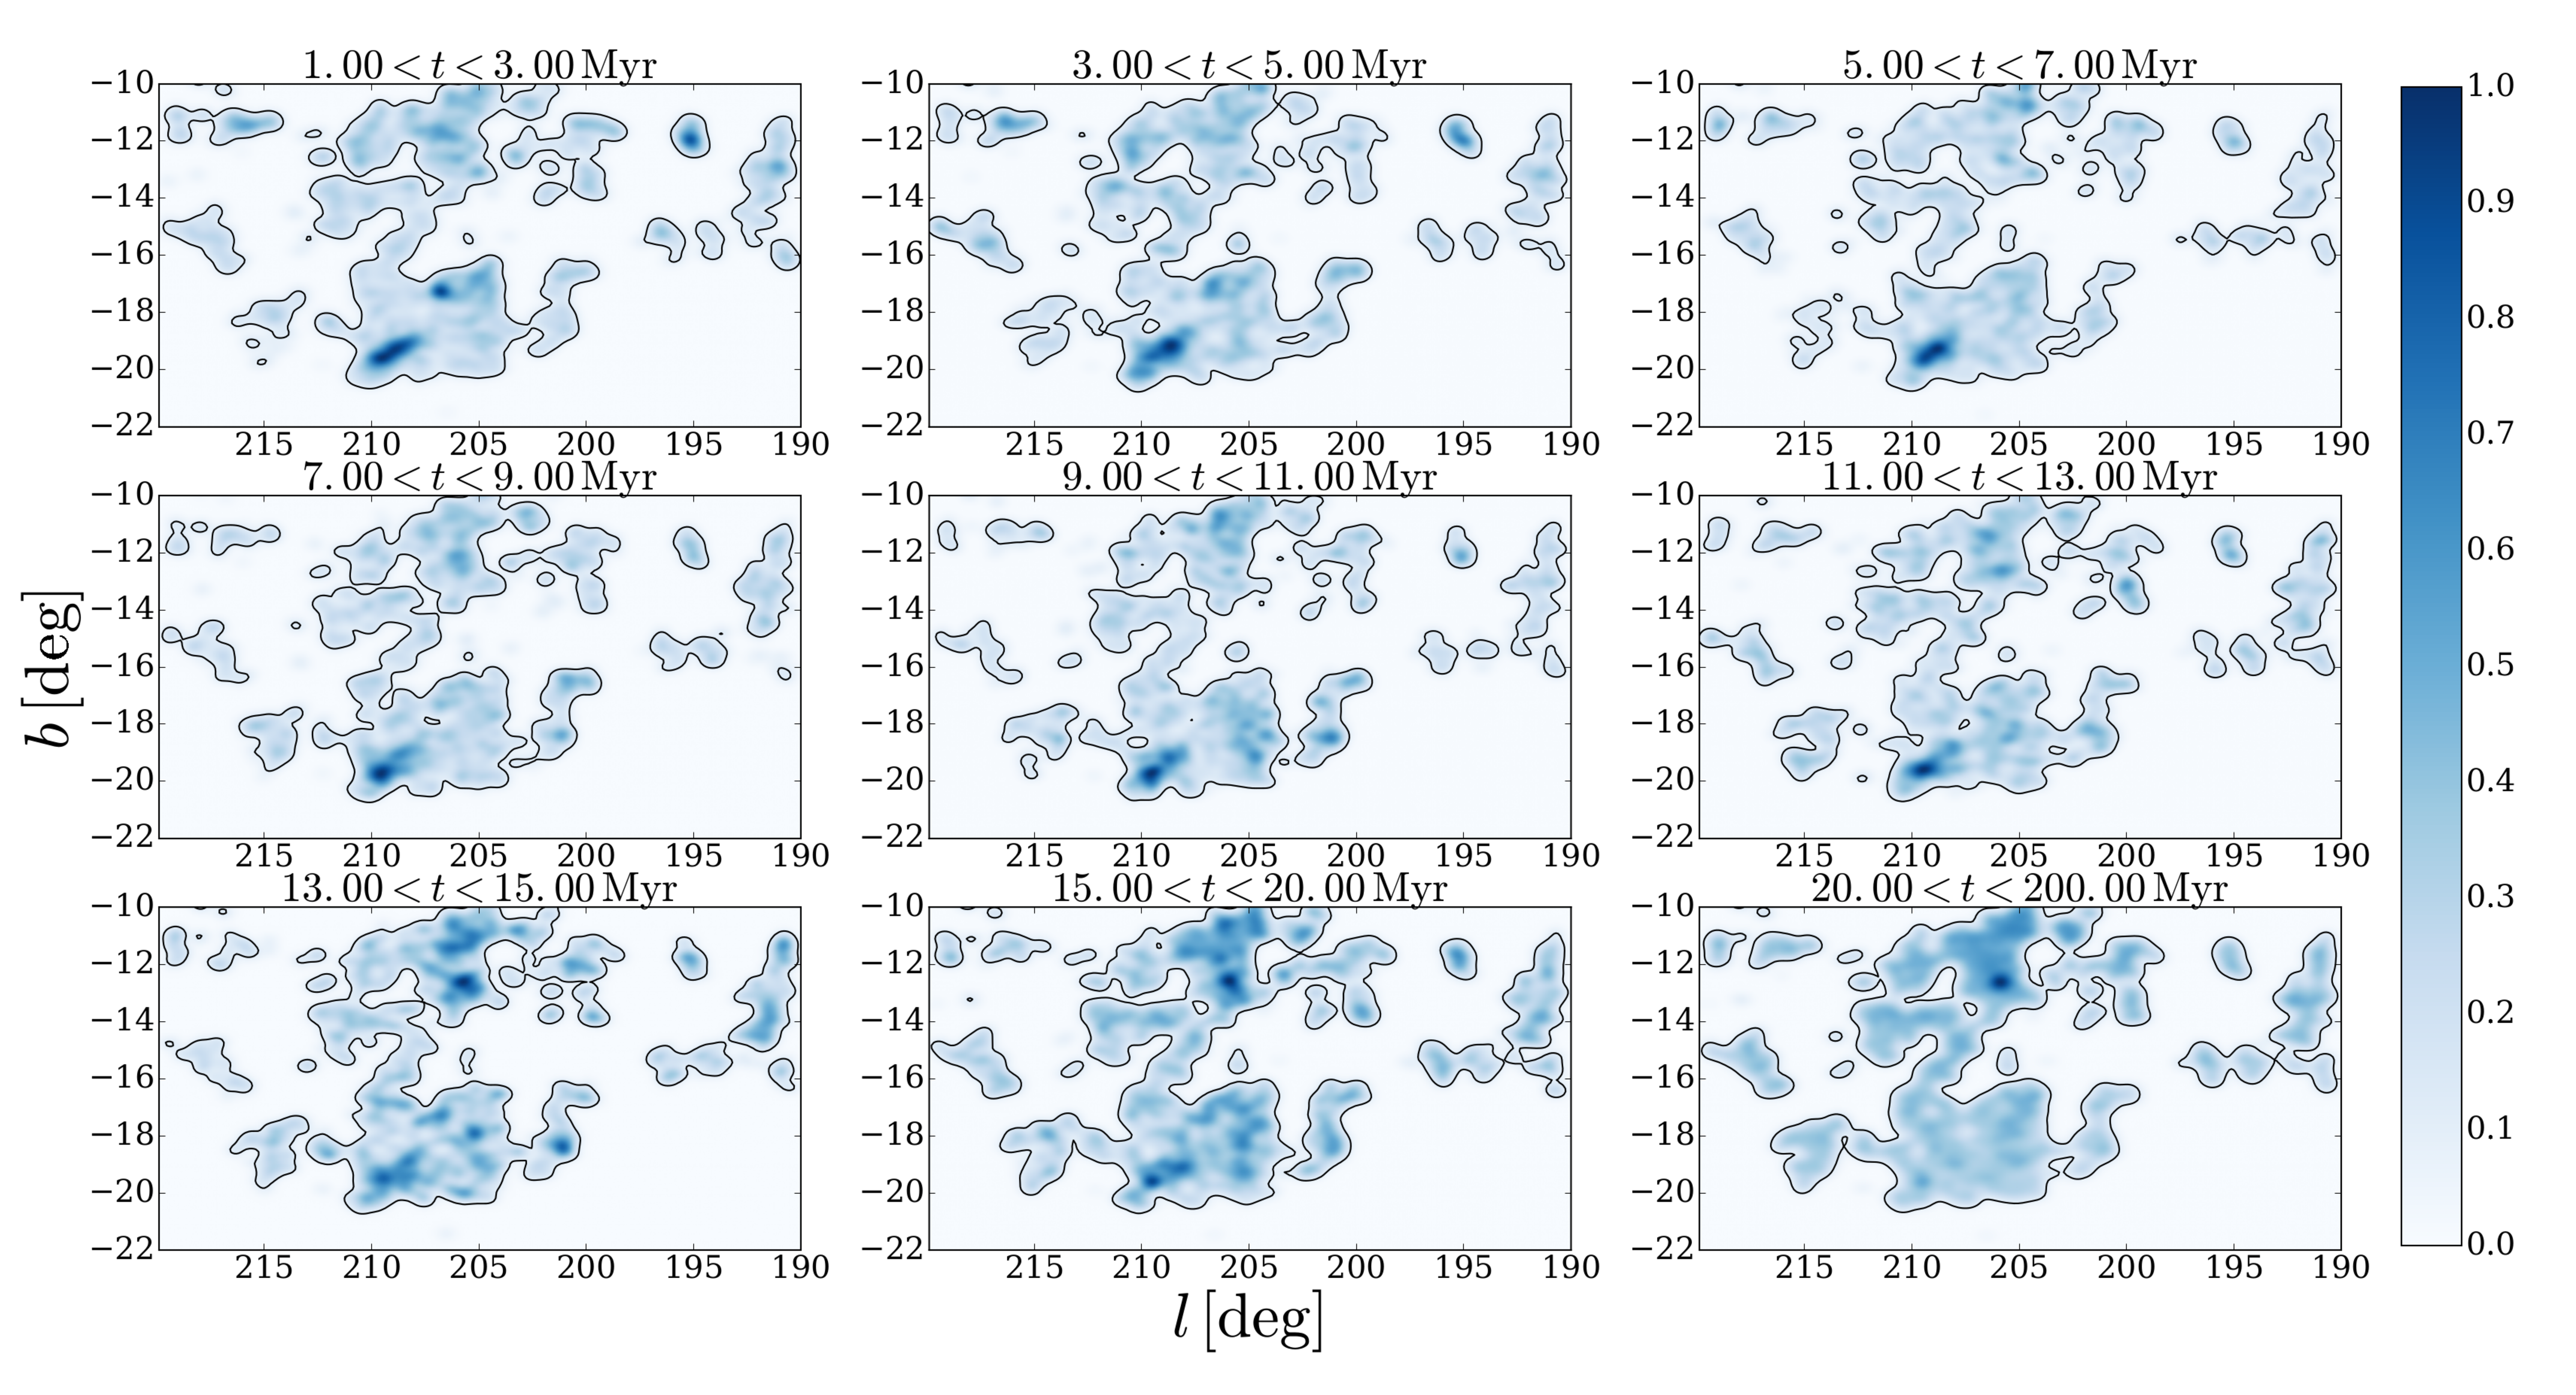
\includegraphics[width = \hsize]{fig7.eps}
\caption{Distribution in the sky of the sources in different age intervals. 
}
\end{figure}

\section{Conclusions}
We studied the stellar population towards Orion and we found evidence for the presence of a young stellar population, at parallax $\varpi \sim 2.65\,  \mathrm{mas}$, loosely distributed around some known clusters: $25$ Ori, $\epsilon$ Ori and $\sigma$ Ori, and NGC 1980 and the ONC. We also found hints of the presence of a parallax gradient going from 25 Ori to the ONC. We estimated the ages of the populations, and we found an age gradient corresponding to the parallax gradient. In particular, the closest stars to the Sun are also the oldest ones.


\tiny 
\textit{Acknowledgements.} This project was developed in part at the 2016 NYC Gaia Sprint, hosted by the Center for Computational Astrophysics at the Simons Foundation in New York City. This  work has made use of data from the European Space Agency (ESA)
mission {\it Gaia} (\url{https://www.cosmos.esa.int/gaia})
, processed by
the {\it Gaia} Data Processing and Analysis Consortium (DPAC,
\url{https://www.cosmos.esa.int/web/gaia/dpac/consortium}).
Funding
for the DPAC has been provided by national institutions, in particular
the institutions participating in the {\it Gaia} Multilateral Agreement.


\normalsize
\bibliographystyle{aa}
\begin{thebibliography}{}

\bibitem[Blaauw  (1964)]{Blaauw1964}
{Blaauw, A.} 1964,
\textit{ARA\&A}, 2, 213 

\bibitem[Bally  (2008)]{Bally2008}
{Bally, J.} 2008,
\textit{Handbook of Star Forming Regions, Volume I}, ed. B. Reipurth, 459 

\bibitem[Bressan (2012)]{Bressan2012}
{Bressan, A., Marigo, P., Girardi, L., et al.} 2012,
\textit{MNRAS}, 427, 127 


\bibitem[Brice\~no (2008)]{Briceno2008}
{Brice\~no, C.} 2008,
\textit{Handbook of Star Forming Regions, Volume I}, ed. B. Reipurth, 838 

\bibitem[Brown  et al. (1994)]{Brown1994}
{Brown, A.G.A., de Geus E.J. \& de Zeeuw P.T.} 1994,
\textit{A \& A}, 289, 101 

\bibitem[Chen  et al. (2014)]{Chen2014}
{Chen, Y., Girardi L. \& Bressan, A.} 2014,
\textit{MNRAS}, 444, 2525 


\bibitem[Da Rio et al. (2014)]{DaRio2014}
{Da Rio N., Tan J. C. \& Jaehnig, K.} 2014,
\textit{ApJ}, 795, 55 

\bibitem[Finkbeiner (2003)]{Finkbeiner2003}
{Finkbeiner, D. P.} 2003,
\textit{ApJS}, 146, 407

\bibitem[Gaia Collaboration (2016a)]{Brown2016}
{Gaia Collaboration, Brown, A.G.A., Vallenari A., et al.} 2016a,
\textit{A \& A}, 595, A2 

\bibitem[Gaia Collaboration (2016b)]{Prusti2016}
{Gaia Collaboration, Prusti, T., de Bruijne, J. H. J., et al.} 2016b,
\textit{A \& A}, 595, A1 

\bibitem[J{\o}rgensen \& Lindegren (2005)]{JL05}
{J{\o}rgensen, B.R. and Lindegren, L.} 2005,
\textit{A\&A}, 436, 127 


\bibitem[Lindegren et al. (2016)]{Lindegren2016}
{Lindegren L., Lammers, U., Bastian U. et al.} 2016,
\textit{A\&A}, 595, A4 


\bibitem[Michalik et al. (2015)]{Michalik2015}
{Michalik, D., Lindegren L., \& Hobbs, D.} 2015,
\textit{A\&A}, 574, A115 


\bibitem[Muench et al. (2008)]{Muench2008}
{Muench, A., Getman K., Hillenbrand L. \& Preibisch, T.} 2008,
\textit{Handbook of Star Forming Regions, Volume I}, ed. B. Reipurth, 483 

\bibitem[Ochsendorf et al. (2015)]{Ochsendorf2015}
{Ochsendorf,B. B., Brown A. G. A., Bally J. \& Tielens, A. G. G. M.} 2015,
\textit{ApJ}, 808, 111

\bibitem[Planck Collaboration (2014)]{Planck2014}
{Planck Collaboration, Abergel, A., Ade, P.A.R, et al.} 2014,
\textit{A \& A}, 571, A11 


\bibitem[Schlafly et al. (2015)]{Schlafly2015}
{Schlafly, E. F., Green G., Finkbeiner D. P.} 2015,
\textit{ApJ}, 799, 116 

\bibitem[Tang et al. (2014)]{Tang2014}
{Tang, J., Bressan A., Rosenfield P. et al.} 2014,
\textit{MNRAS}, 445, 4287 


\bibitem[Valls-Gabaud (2014)]{Valls-Gabaud2014}
{Valls-Gabaud, D.} 2014,
\textit{EAS Publication Series, Vol. 65}, 225, 265 


\end{thebibliography}


\end{document}

